\section{Evaluering}

\subsection{Lydkredsl�b sammenholdt med h�jttaler}
Peter V�d�le Clausen har analyseret den del af NXT'ens lydkredsl�b, der kommer f�r h�jttaleren. Iflg. ham har NXT'en ikke en egentlig A/D-converter, men benytter sig af Pulse Width Modulation (PWM) til at frembringe lyden. Konverteringen fra PCM til PWM bevirker at der genereres en m�ngde h�jfrekvens st�j, hvilket i NXT'en fjernes med et lavpas-filter. Peter V�d�le Clausen har vha. et sinus-sweep m�lt frekvensresponset p� kredsl�bet samt det analoge filter, vist i figur \ref{circuit}.

% kredsl�b og filter
\begin{figure}
\begin{center}
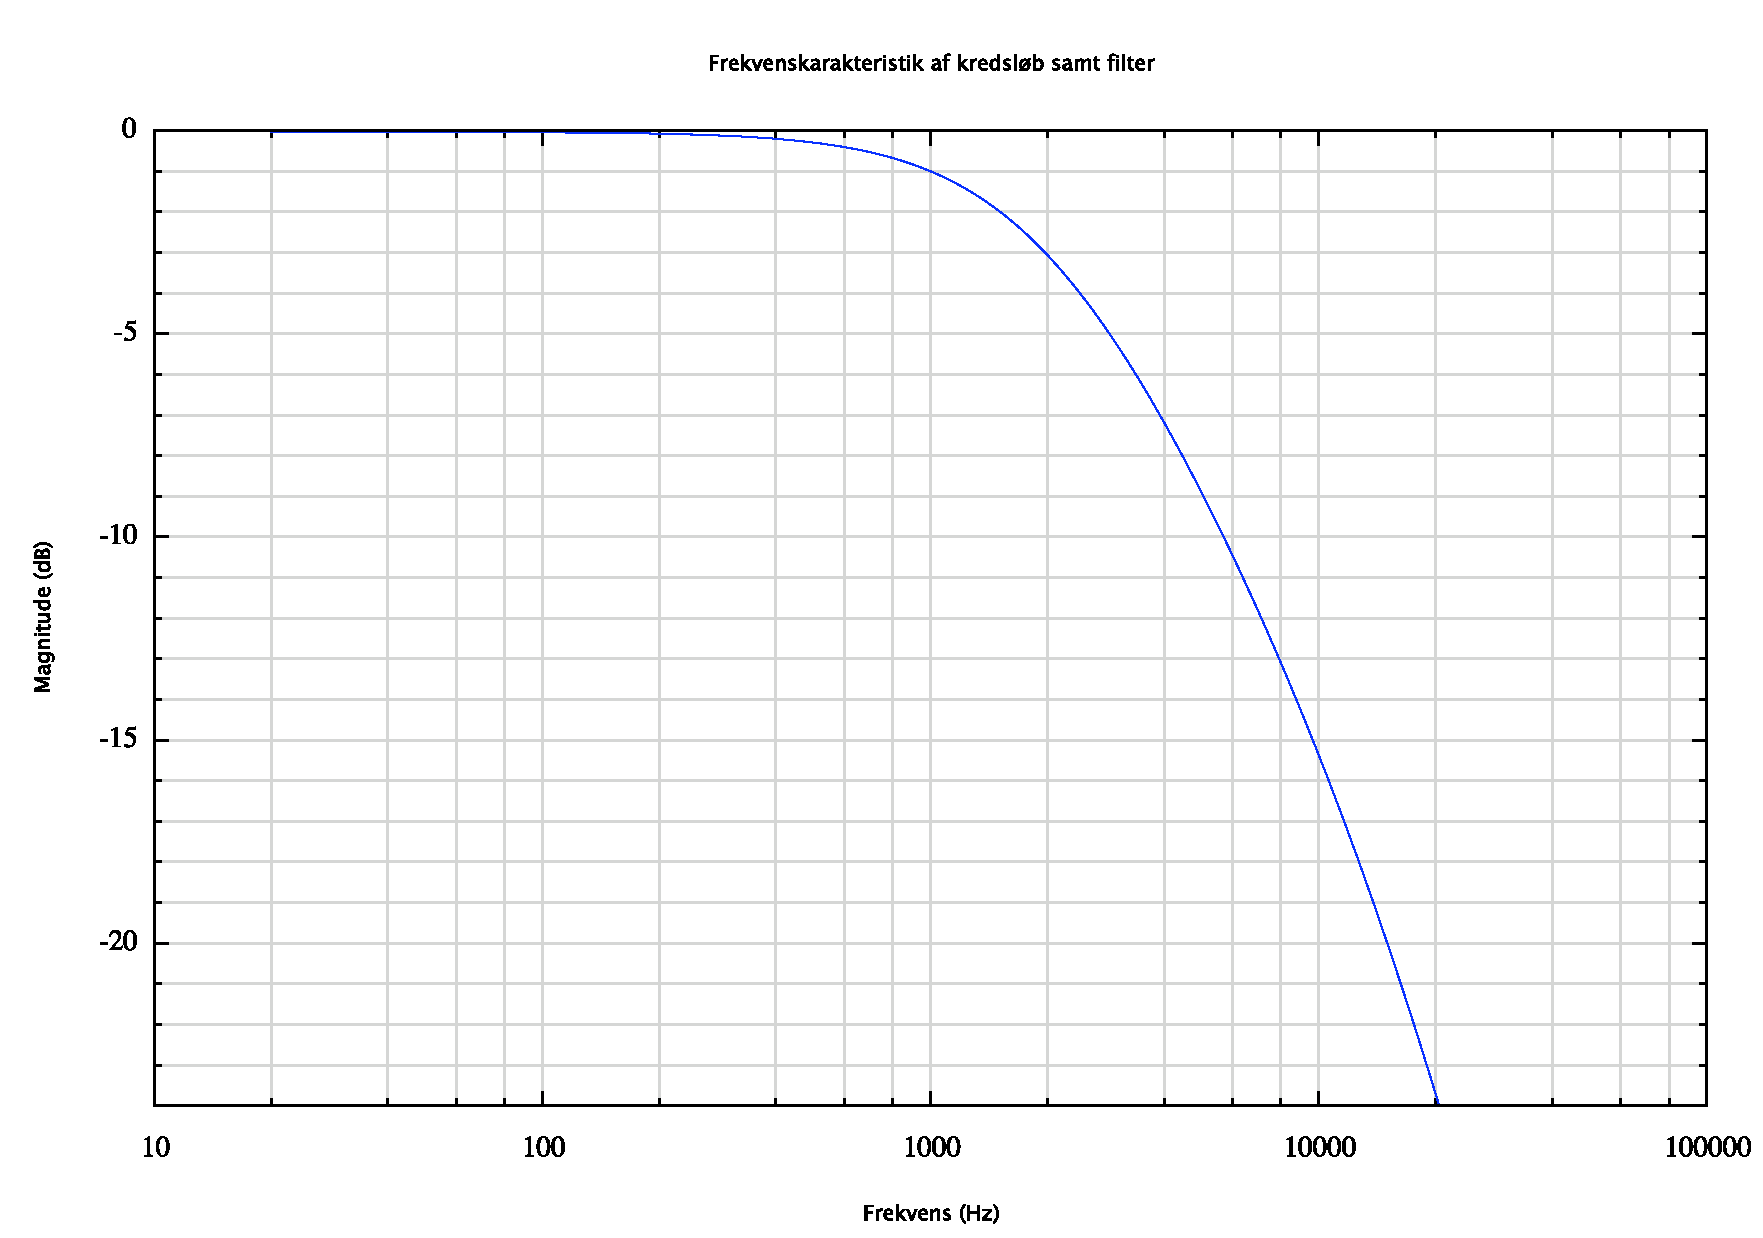
\includegraphics[width=12cm]{circuit-filter.pdf}
\end{center}
\caption{Digitalt kredsl�b samt analogt filter i NXT}
\label{circuit}
\end{figure}

%

Som det fremg�r af figur \ref{circuit}, bevirker NXT'ens kredsl�b sammen med det analoge filter et fald p� 3 dB ved omkring 2 kHz, mens h�jttaleren f�rst begynder at respondere ved 600 Hz. Som det fremg�r af figur \ref{onaxis}, har h�jttaleren med kabinet endvidere et dyk omkring de 2 kHz. 

Med NXT'en f�lger en r�kke lydfiler med tale, og da frekvensen af forst�elig tale ligger mellem 400 og 3500 [henvisning?] Hz, vil NXT'en sikkert fint kunne frembringe dette.

generelt, hvad egner h�jttaleren sig til (musik/bip-lyde/taler)
Egner h�jttaleren sig til det den er t�nkt til?

Forslag til korrigering osv
